%\documentclass[draft]{ws-procs9x6}
\documentclass{ws-procs975x65}
\usepackage{comment}
\usepackage{subfigure}
\usepackage{color}
\usepackage{epsfig}
\usepackage{times}
\usepackage{url}
\begin{document}

\title{Improving local multiple alignment of interspersed DNA repeats with gapped extension}

\author{Todd J. Treangen$^\dag*$}

\address{Dept. of Computer Science, Technical Univ. of Catalonia\\
Barcelona, Spain\\
$^*$E-mail: treangen@lsi.upc.edu}

\author{Aaron E. Darling$^\dag*$}

\address{Institute for Molecular Bioscience, Univ. of Queensland\\
Brisbane, Australia\\
$^*$E-mail: a.darling@imb.uq.edu.au}


\author{ Mark A. Ragan}

\address{Institute for Molecular Bioscience, Univ. of Queensland\\
Brisbane, Australia\\
}

\author{ Xavier Messeguer}

\address{Dept. of Computer Science, Technical Univ. of Catalonia\\
Barcelona, Spain\\
}
\maketitle
{\center \scriptsize $^\dag$ These authors contributed equally to this work \\}

\abstracts{
The identification of homologous DNA is a fundamental building block of comparative genomic and molecular evolution studies.  To date, methods to identify and align all homologous nucleotides in one or more genomes have suffered poor scalability and limited accuracy.  We propose a novel method that couples a gapped extension heuristic with a previously described efficient filtration method for local multiple alignment.  During gapped extension, we use the MUSCLE implementation of progressive multiple alignment with iterative refinement.  The resulting gapped extensions are global multiple alignments, and often contain alignments of unrelated sequence.  We detect and remove such undesirable alignments using a hidden Markov model to predict the posterior probability of unrelated sequence.  We evaluate the performance of our method and previous approaches on a hybrid dataset of real genomic DNA with simulated interspersed repeats.  Our method compares favorably to existing methods in terms of sensitivity, positive predictive value, and localizing boundaries of homology.
The described methods have been implemented in the free, open-source \texttt{procrastAligner} software, available from \url{http://somewhere.net}\textbf{FIXME: find a permanent home for procrastAligner}
}

\keywords{sequence alignment, local multiple alignment, interspersed repeats, gapped extension}

\section{Introduction}
The importance of accurate homology identification to comparative genomics should not be underestimated\cite{Kumar07}. To date, pairwise local sequence alignment methods\cite{ref-blastz,ref-ssearch} have been the prevailing technique to identify homologous nucleotides.  When more than two copies of a homologous sequence element are present in the data, pairwise homology detection methods generate a listing of all possible pairs of homologous elements in the form of pairwise local alignments.  Apart from the obvious inefficiency of considering all pairwise homology relationships, a collection of pairwise alignments is not ideal because they are rarely amenable to comparative genomic and phylogenetic analysis without further processing into a multiple alignment.

Local pairwise alignments can be merged to create a multiple alignment by a variety of methods\cite{ref-tba,ref-aba,ref-dialign,ref-related1}. Such methods commonly assume that pairwise homology relationships are transitive, such that if nucleotide $a$ is homologous to nucleotide $b$, and $b$ is to $c$, then $a$ must also be homologous to $c$.  Thus, in order to merge pairwise alignments, such methods must tackle the challenging problem of resolving inconsistent transitive homology relationships.  Multiple alignment has been demonstrated to be more accurate than pairwise alignment, especially when dealing with a large number of divergent sequences\cite{ref-mlagan,ref-aubergene}.  As the number of homologous sequences grows, we might expect that the number of inconsistent relationships in a collection of pairwise alignments would grow quadratically, whereas a direct multiple alignment method would provide an increasingly accurate alignment.  Highly repetitive regions in the input sequences can cause serious efficiency problems for pairwise methods, as they create $O(r^{2})$ pairwise alignments in the presence of a repeat with $r$ copies.  Mammalian Alu repeats and IS elements in microbes are two common examples of the overwhelming abundance of repetitive sequence in whole genomes.

Local multiple alignment has the inherent potential to avoid pitfalls associated with pairwise alignment. Although optimal multiple alignment under the SP objective function remains intractable\cite{ref-wangjiang}, progressive alignment heuristics offer excellent speed and accuracy\cite{ref-clustalw,ref-tcoffee} especially when combined with tree-independent iterative refinement\cite{ref-muscle}, or probabilistic consistency measures\cite{ref-probcons}. Rather than merging pairwise alignments, why not exploit years of research into multiple alignment heuristics by directly constructing a multiple alignment? We thus present a novel heuristic for directly computing local multiple alignments via gapped extension of chained seed matches.

\section{A heuristic for local multiple alignment}
Our method for computing local multiple alignments exploits the MUSCLE multiple alignment algorithm to compute gapped extensions of ungapped multi-match seeds (see Figure~\ref{fig-main}). Gapped alignments arise when extending seeds to fully capture surrounding sequence homology. Our method assumes that a fixed number of nucleotides flanking a seed match are likely to be homologous and computes a global multiple alignment on the flanking region.  Our assumption of flanking homology often proves to be erroneous and results in an alignment of unrelated sequences.  In the context of \textit{local} multiple alignment, the fundamental problem with such an approach is that current methods for progressive alignment with iterative refinement compute \textit{global} alignments, i.e. they implicitly assume that input sequences are homologous over their entire length.  To resolve the problem, we employ a hidden Markov model which detects unrelated regions embedded in the global multiple alignment.  Unrelated regions are then removed from the alignment and the local-multiple alignment is trimmed to reflect the updated boundaries of homology.

Our method for local multiple alignment, as depicted in Figure~\ref{fig-main},
has seven primary steps: (1) identifying multi-match seeds in the input sequence, (2) chaining individual seeds, (3) multiple alignment of regions between chained seeds, (4) gapped extension of seed chains (5) detection of unrelated regions using a hidden Markov model, (6) application of transitive homology relationships, and (7) unalignment of any unrelated sequence to produce final local multiple alignment.  Steps 2-7 are applied repeatedly to seeds identified in step 1 to produce local multiple alignments of all homologous nucleotides in the input sequence.


\begin{figure}[p]
\begin{center}
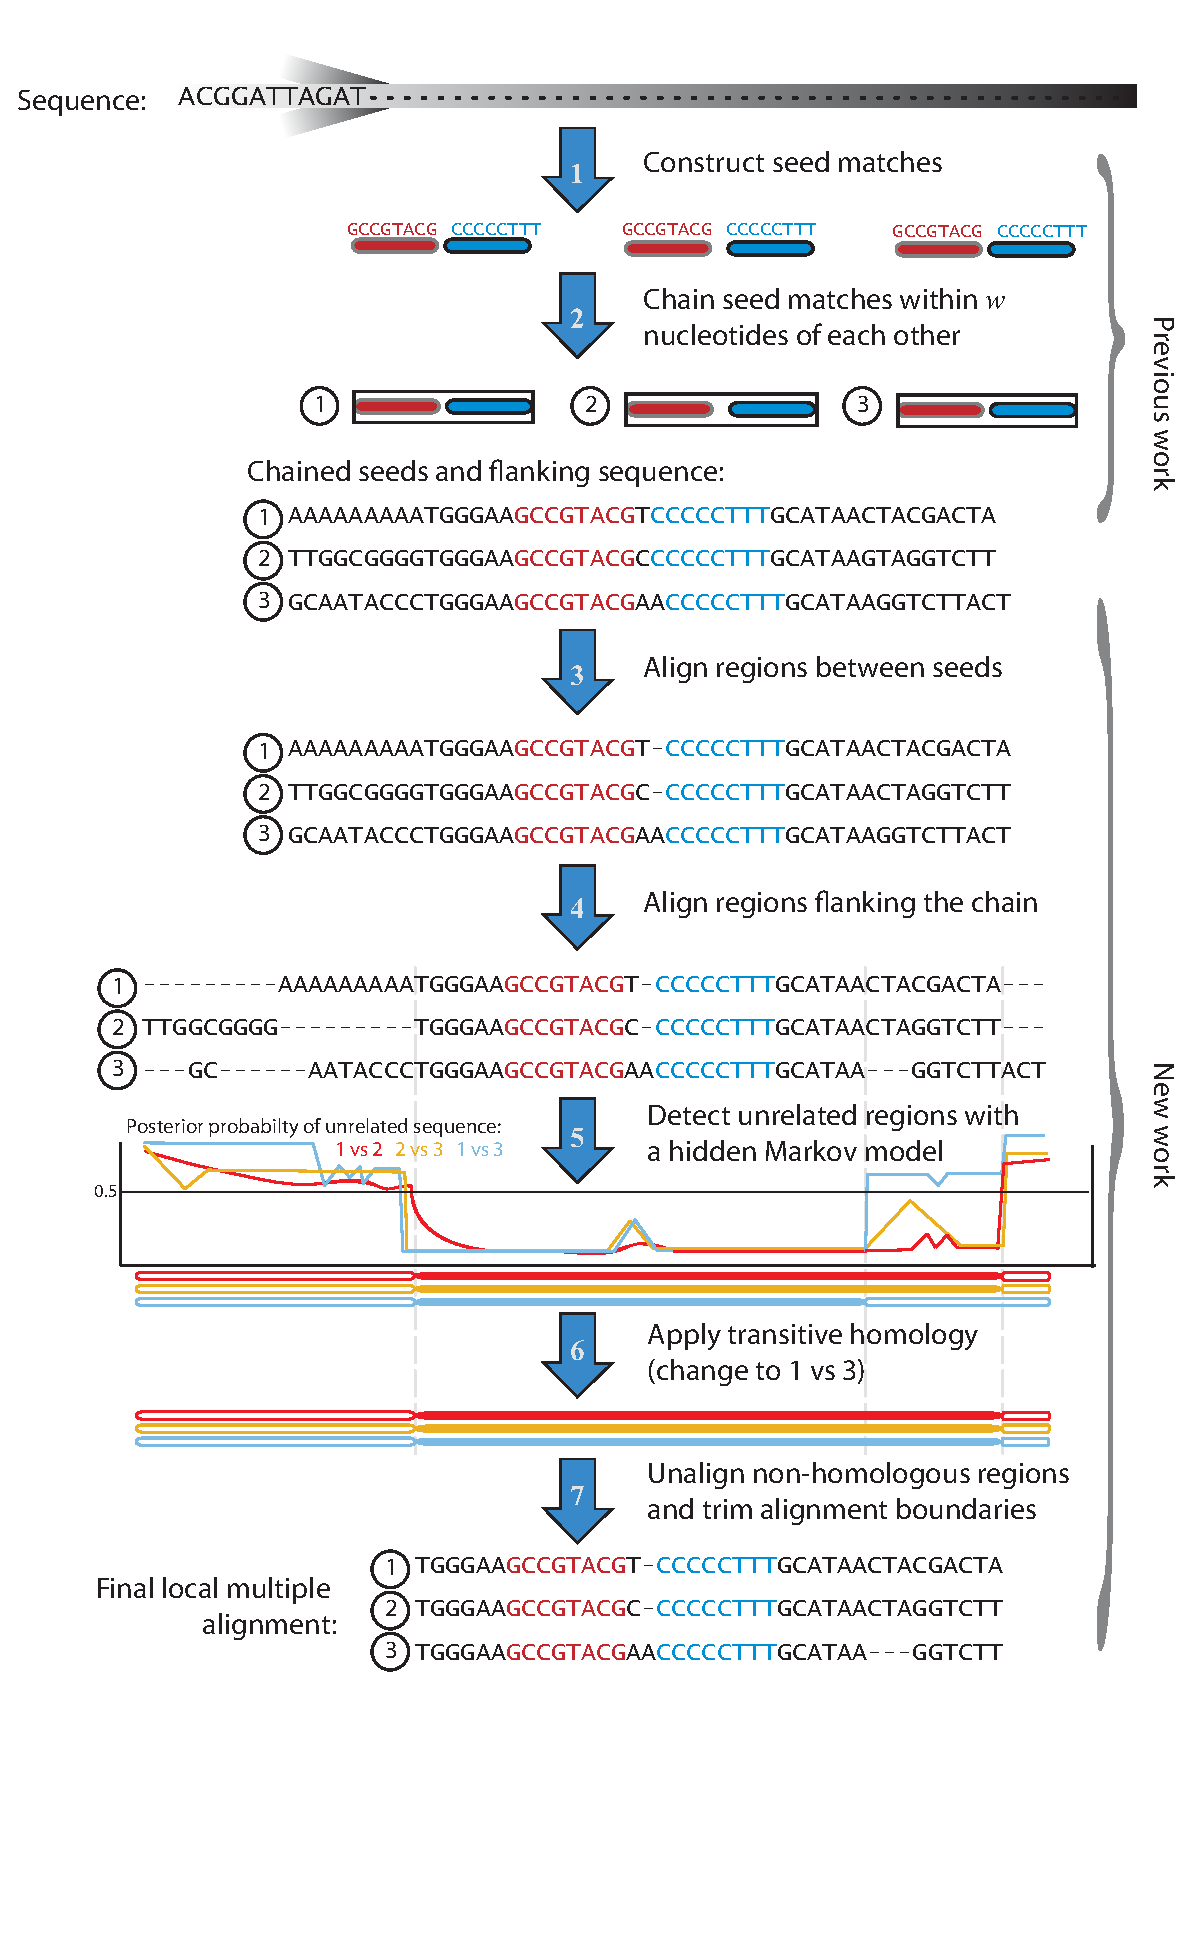
\epsfig{file=./figures/extension.eps,width=4.1in}
%\subfigure[Visual representation of our algorithm]{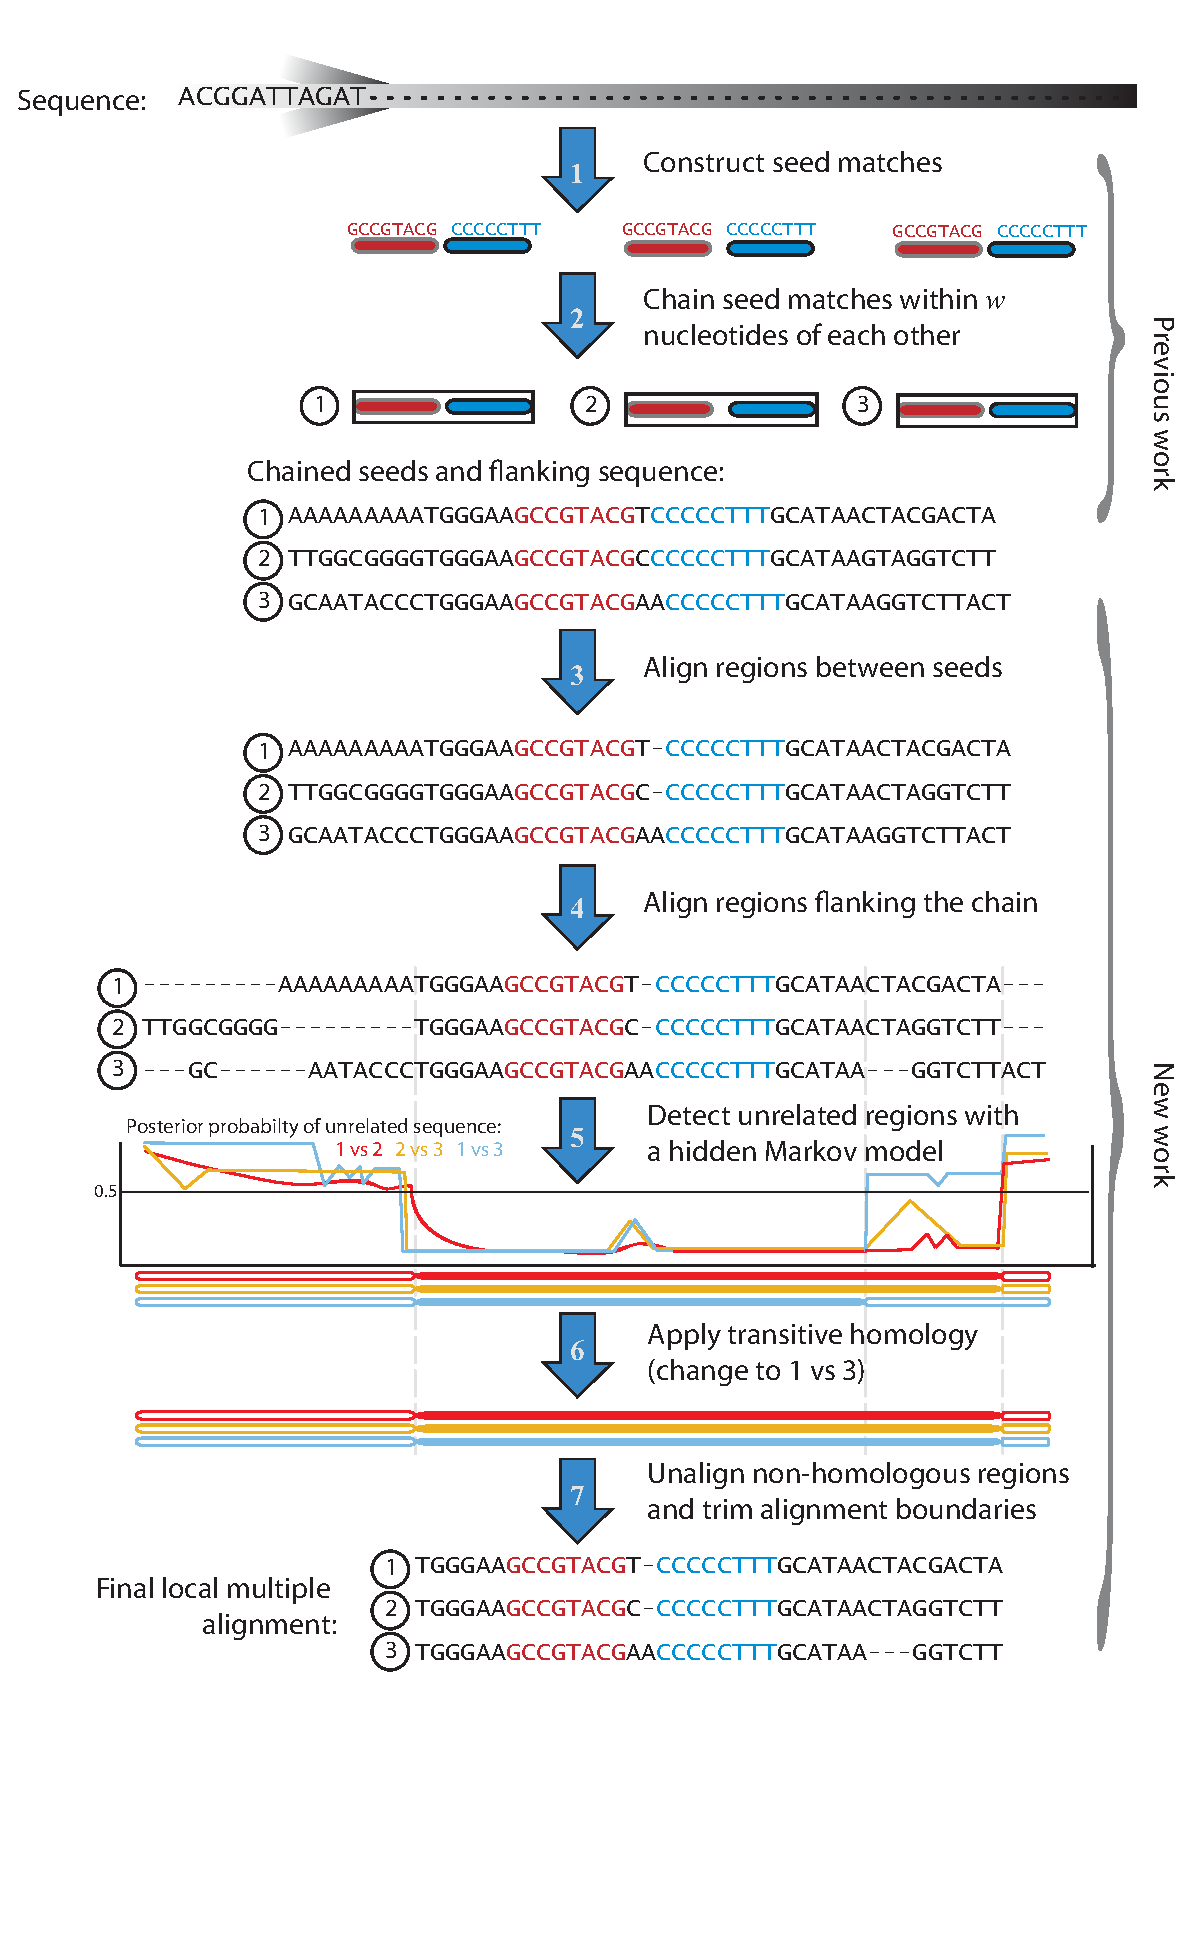
\epsfig{file=./figures/extension.eps,width=3.0in}}
%\subfigure[Flowchart of the algorithmic process ]{ 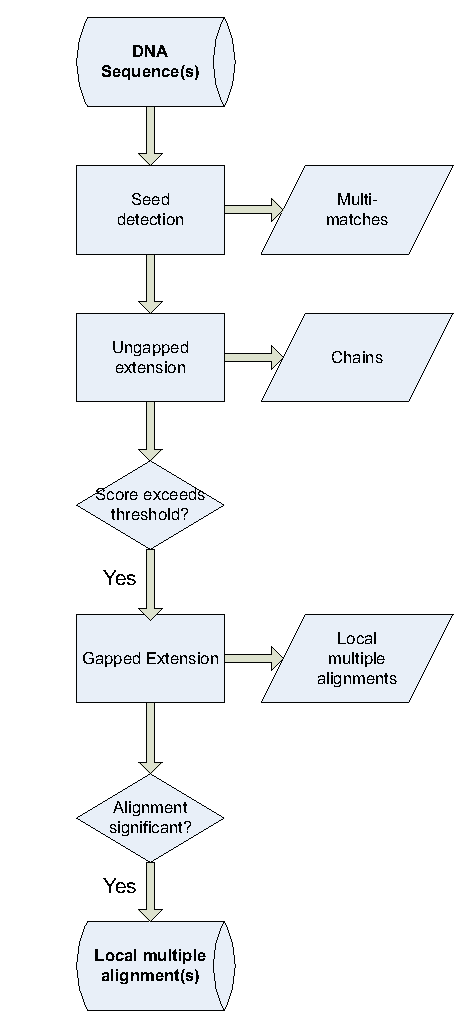
\epsfig{file=./figures/flowchart.eps,width=1.7in}}
\end{center}
\vspace{-1.6cm}
\caption{Overview of the method, starting with an input sequence and ending with a set of local multiple alignments. First we (1) detect multi-matches in the input sequence(s) using palindromic spaced seeds, then we perform (2) chaining and extension of all multi-matches within $w$ nt of each other.  In the present example, one chain exists and contains two matches each with three match components labeled 1, 2, and 3.  We then perform gapped alignment of the region between chained matches (3).   In step (4), we perform a gapped extension by computing a global multiple alignment on the regions to the left and right of each chain component.  The resulting alignment may contain unrelated sequence, so in step (5) we apply a hidden Markov model to detect poorly aligned regions indicative of unrelated sequence.  Step (6) computes transitive homology relationships to ensure a consistent alignment and aid detection of divergent homologous sequences.  Finally, in step (7) we unalign regions found to be non-homologous.  If we find after step (2) that the alignment boundaries have been extended, we return to step (4) for another round of chaining.}
\label{fig-main}
\end{figure}

\subsection{Extracting multi-matches from the input sequence}
Given a sequence $\mathcal{S}=s_1, s_2,\dots, s_N$ of length $N$
defined over an alphabet $\{A,C,G,T\}$, our goal is to identify all
significant local multiple alignments on subsequences of $\mathcal{S}$. Our
method first extracts candidate ungapped alignments, or multi-matches,
among subsequences in $\mathcal{S}$, denoted as $\mathbf{M}$. To extract multi-matches from the input sequence, we utilize a palindromic spaced seed pattern, which is analyzed at each position in the input sequence.  Previously we have demonstrated that palindromic spaced seeds offer good efficiency and reasonable sensitivity on a variety of input sequences\cite{ref-procrast}.
We refer the number of matching regions in $\mathcal{S}$
by a given match $M_i \in \mathbf{M}$ as the
\textit{multiplicity} of $M_i$, denoted as $|M_i|$. We refer to each
matching region of $M_i$ as a \textit{component} of $M_i$. Our algorithm has an important limitation on the matches in
$\mathbf{M}$: no two matches $M_i$ and $M_j$ may have the same
left-end coordinate, except for the identity case when $i=j$.  This constraint
has been referred to by others as \textit{consistency} and
\textit{transitivity}\cite{ref-transitivity} of matches.

\subsection{Creating chains of multi-matches}
Once a list of multi-matches has been generated, we employ an efficient chaining and filtration algorithm to identify overlapping and nested chains of multi-matches\cite{ref-procrast}. In order to chain process each region of sequence $\mathcal{O}(1)$ times, matches are prioritized for chaining in order of decreasing multiplicity.  Our method chains seed multi-matches of the same multiplicity $M_{i}$ occurring within $w$
characters of each other.
When a multi-match can no
longer be chained without including a gap larger than $w$
characters, neighboring \textit{subset}
matches within $w$ characters are identified. Each 
neighboring subset match is then \textit{linked} to the chained match. We refer to the
chained match as a \textit{superset} match. Rather than immediately
extend the subset match(es), we \textit{procrastinate} and extend
the subset match later when it has the highest multiplicity of any
match waiting to be extended. When chaining a match with a linked
superset, we immediately include the entire region covered by the linked superset
match and thus eliminate the need to re-examine sequence already covered by
a previously chained match.  

\subsection{Gapped extension of high scoring chains}

After chaining a multi-match $M_i$, we perform gapped alignment on all collinear regions located between two adjacent components to generate unextended local multiple alignments. We first evaluate the chain to decide whether expending computational resources on gapped extension will be worthwhile. We can require that two or more seeds be present in the chain and use lower seed weights ($k$), a technique which has previously been proven successful\cite{ref-blastz,ref-gappedblast,ref-blat}.  To perform a gapped extension in each direction, we use MUSCLE to align a fixed number of nucleotides ($l$) to the left and right of the current local multiple alignment.
Small values of $l$ restrict the alignment search space, while larger values require more computation but are potentially more sensitive.  We have experimentally determined that setting $l$ based on multiplicity ($l = 70e^{-0.01*|M_{i}|}$) offers a good tradeoff between speed and sensitivity.  The resulting extension window is small for high multiplicity chains ($|M_{i}|\geq 30$), keeping the alignment search space tractable.
%\begin{equation}
% \max(w, \sqrt{(\max(150^{2}-(2*|M_{i}|)^{2},0)}));
%\end{equation}

\subsubsection{Identifying unrelated regions}
\begin{figure}[t]
\centering 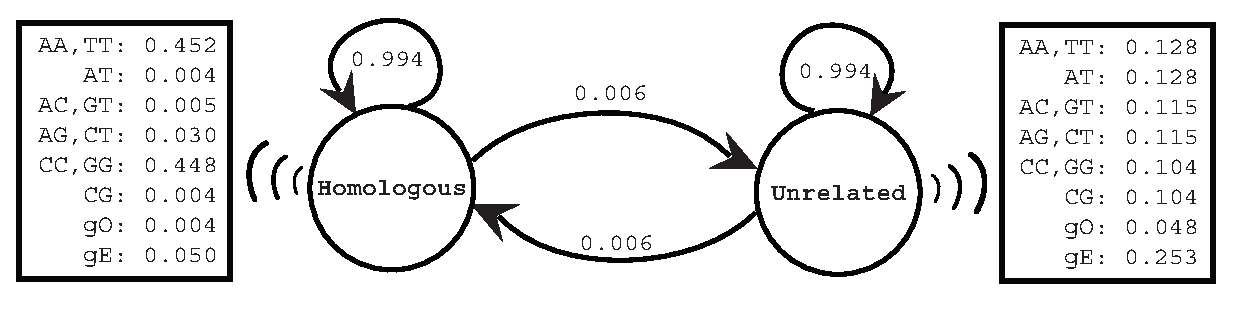
\epsfig{file=./figures/hmm.eps,width=4.8in}
\caption{Hidden Markov model used to detect pairwise alignments of unrelated sequence. The HMM has states which model alignment columns containing homologous and unrelated sequence.  Emissions correspond to alignment columns, for example \texttt{AA} indicates A aligned to A.  gO indicates gap open and gE gap extend. Alignment columns are treated as strand-symmetric, so that AC also indicates CA and the reverse complements TG and GT.}
\label{fig-hmm}\vspace{-0.2cm}
\end{figure}
The MUSCLE alignment software dutifully reports the highest scoring global multiple alignment of input sequences, regardless of whether they are related by common ancestry. As a consequence of the gapped extension process, it is likely that we forcibly align unrelated sequence. We have configured a hidden Markov model (Figure ~\ref{fig-hmm}) to detect alignments of unrelated sequence. The HMM consists of two hidden states, Homologous and Unrelated. The observable states are the pairwise alignment columns, which are all possible pairs in $\texttt{{\{A,G,C,T,-\}}}$ with strand and species symmetry, i.e. \texttt{AG=GA=TC=CT}.  The emission probabilities for each possible pair of aligned nucleotides were extracted from the HOXD substitution matrix presented by Chiaramonte \textit{et al} 2002\cite{hoxd}. We solved for the emission frequencies in the homologous and unrelated state using the same equation used in to calculate the values of the HOXD substitution matrix on 47.5\%G+C content sequence\cite{hoxd}:
\begin{equation}
s(x,y)= \log_{2}{\Bigg(\frac{p(x,y)}{q_{1}(x)q_{2}(y)}\Bigg)}
\end{equation}
where $p(x,y)$ is the fraction of the observed aligned pairs of nucleotides $x$ and $y$ in the training set used and $q_{1}(x)$ and $q_{2}(x)$ denote the background frequencies of $x$ and $y$, respectively. Chiaramonte \textit{et al.} scaled the resulting $s(x,y)$ values by an unreported value $\psi$ so the largest was 100, with the rest rounded to the nearest integer.  Given that the training data has $47.5\%G+C$ content and considering strand and species symmetry, we can compute emission frequencies for the Unrelated state of our HMM: \begin{center}$U_{AA}=U_{AT}=U_{TA}=U_{TT}=(\frac{f_{AT}}{2})(\frac{f_{AT}}{2}) = 0.06890625$ \\
$U_{CC}=U_{CG}=U_{GC}=U_{GG}=(\frac{f_{GC}}{2})(\frac{f_{GC}}{2}) = 0.05640625$ \\
$U_{AC}=U_{AG}=U_{TC}=U_{AG}=(\frac{f_{AT}}{2})(\frac{f_{GC}}{2}) = 0.06234375$ \\
$U_{CA}=U_{CT}=U_{GA}=U_{GT}=(\frac{f_{GC}}{2})(\frac{f_{AT}}{2}) = 0.06234375$ \\
\end{center}

Where $f_{GC}=0.475$ and $f_{AT}=0.525$ are background frequencies of G/C and A/T, respectively.
Then we derive emission probabilities for the Homologous state as, for example:
\begin{equation}
\log_{2}\bigg(\frac{H_{AA}}{U_{AA}}\bigg) = \frac{91}{\psi},
\end{equation}
where $\frac{1}{\psi}$ is the unknown scaling factor used normalize $H_{CC}$ to 100. The full list of equations follow:
\begin{center}$\log_{2}\bigg(\frac{H_{AC}}{U_{AC}}\bigg) = \frac{-114}{\psi},$
$\log_{2}\bigg(\frac{H_{AG}}{U_{AC}}\bigg) = \frac{-31}{\psi}$ \\
$\log_{2}\bigg(\frac{H_{AT}}{U_{AC}}\bigg) = \frac{-123}{\psi},$
$\log_{2}\bigg(\frac{H_{CG}}{U_{CC}}\bigg) = \frac{-125}{\psi}$ \\
$\log_{2}\bigg(\frac{H_{AA}}{U_{AA}}\bigg) = \ \ \ \frac{91}{\psi},$
$\log_{2}\bigg(\frac{H_{CC}}{U_{CC}}\bigg) = \ \ \ \frac{100}{\psi}$ \\
\end{center}

The system of six equations has seven free variables.  Moreover, the $H_{xy}$ must sum to 1 to make a probability distribution:
\begin{equation}
H_{AA} + H_{AC} + H_{AG} + H_{AT} + H_{CC} + H_{CG} = 1
\end{equation}
%$0.03072937146$
%$32.54215601$
We can solve the above six equations for $H_{xy}$ and substitute the resulting expressions in to the
normalizing equation to solve for $\psi$. For the HOXD matrix the scaling factor $\psi=32.5421$. Given $\psi$, we can calculate values for all $H_{xy}$ in the HMM.

Emission frequencies for nucleotide substitutions can be derived from any strand/species symmetric nucleotide substitution matrix, but gap open and extend frequencies can not.  To empirically estimate values for the unrelated state we aligned a 10kb, 48\% GC content region taken from \emph{E. coli} CFT073 (Accession AF447814.1, coordinates 37,300-38,300) with an unrelated sequence.  We generated an unrelated sequence with identical nucleotide composition by reversing the extracted sequence without complementation.  We then forced an alignment with MUSCLE and counted the number of gap open and gap extend columns in the alignment of unrelated sequences.  Gap open and extend frequencies for the homologous state were estimated by constructing an alignment of 10kb of orthologous sequence shared among a pair of divergent organisms.  We aligned the 48\%GC segment between genes \textit{fruR} and \textit{secA} from \textit{E. coli} K12 (Accession U00096.21) and \emph{Y. pestis} CO92 (Accession AL590842.1). We add the empirically derived gap-open and extend frequencies for each state and normalize the emission frequencies to a probability distribution.  The resulting emission probabilities are reported in Figure~\ref{fig-hmm}.

Using the empirically derived transition and emission probabilities, we apply the posterior HMM decoder implemented in Gerton Lunter's HMMoC software\cite{hmmoc} to compute the posterior probability that each alignment column represents homologous sequence.  Columns with a p.p. below 0.5 are considered to be unrelated.  We then apply the transitive homology principle to our predictions, resulting in a final set of consistent homology predictions.  See Figure~\ref{fig-main}, steps 5 and 6 for an example. We trim the alignment to exclude all columns beyond the Homologous state. If the original boundaries were improved, we trigger another round of chaining (and consequently another round of extension) in the same direction on the currently active match $M_i$.  When gapped extension fails to improve boundaries in one direction, extension in the other direction is attempted until no further extension is possible.


\section{Results}
\begin{figure}[t]
\centering 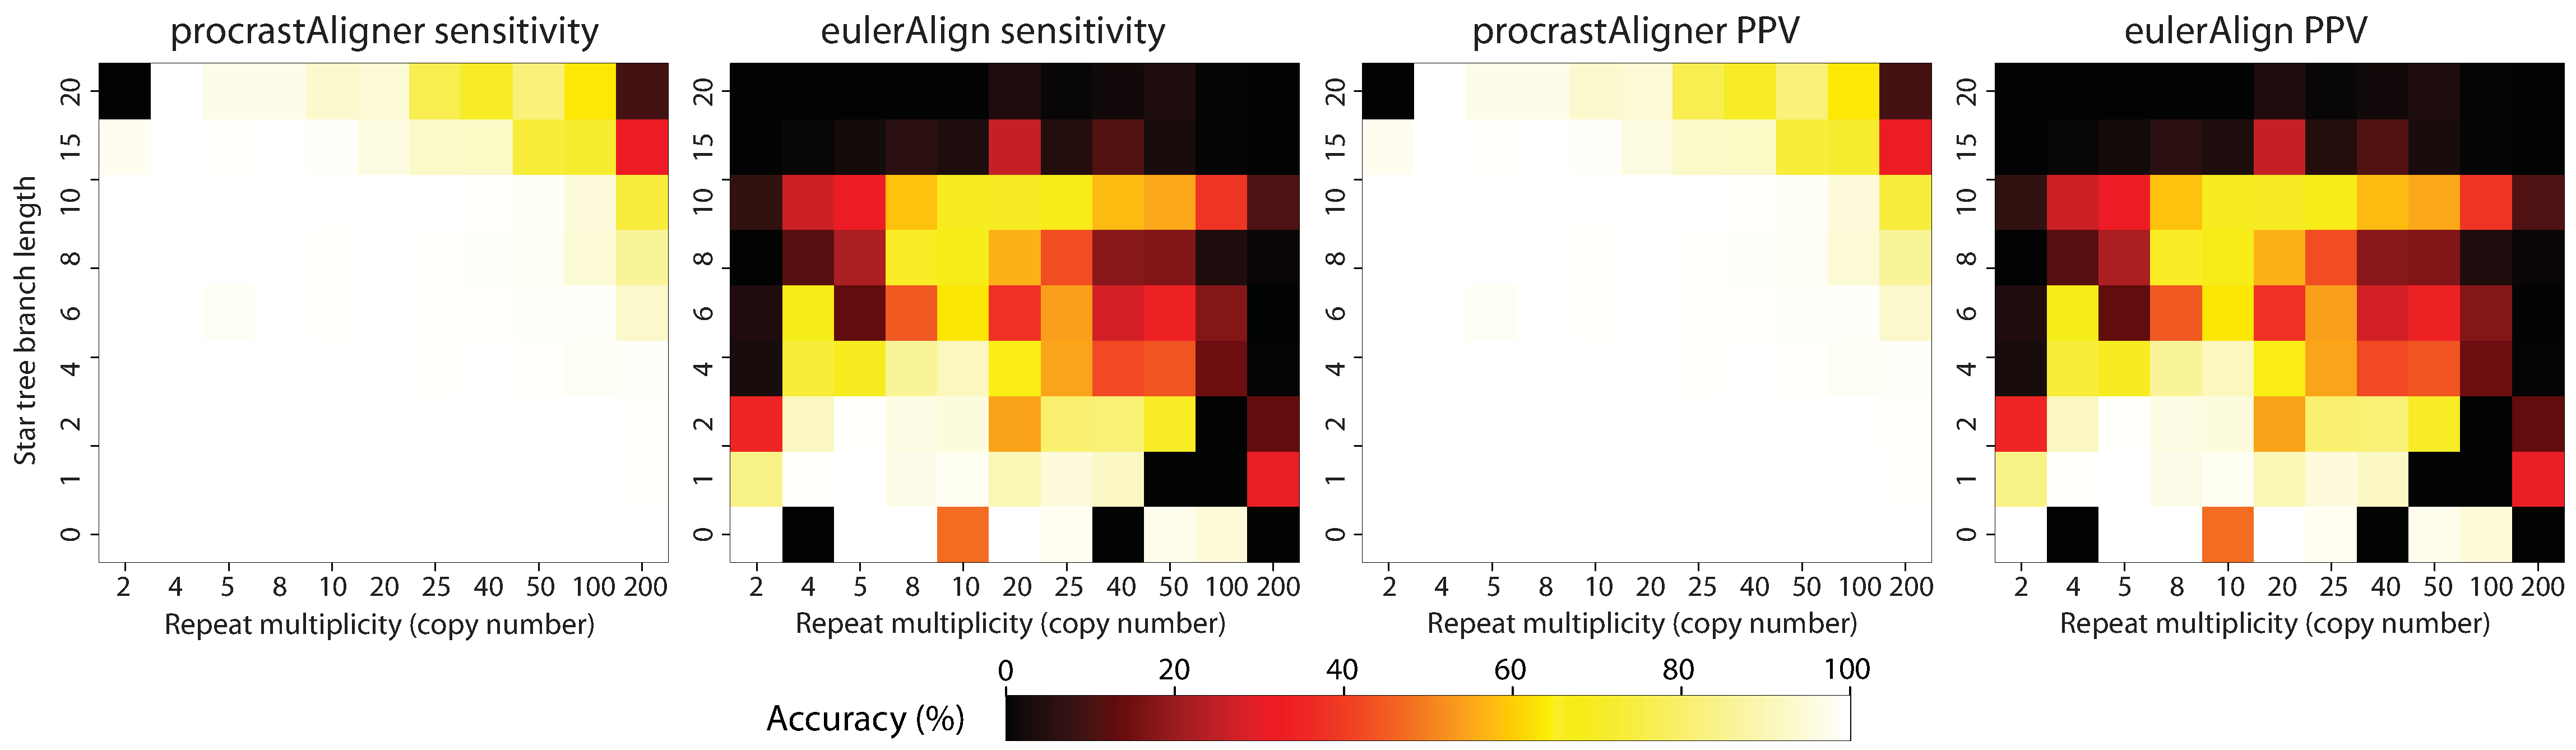
\epsfig{file=./figures/repeat_accuracy.eps,width=5.0in}
\caption{Accuracy of \texttt{procrastAligner} and \texttt{eulerAlign} in recovering simulated repeat families implanted into the \textit{Mycoplasma genitalium} genome.  Sum-of-pairs nucleotide sensitivity and positive predictive value (PPV) were measured for 110 combinations of branch length and multiplicity.  Two replicates of each simulation were performed and
average accuracy values are shown here.  White points indicate perfect alignment of the simulated repeat family.  Black points indicate the program completely failed to recover any portion of the repeat family.  Mutations per site can be calculated by multiplying branch length by the fixed substitution rate of 0.085, and indel rate of 0.015.
For example, at branch length 20 there are 1.7 substitutions per site and 0.3 indels per site.
From the figure, it is apparent that \texttt{procrastAligner} performs well at higher mutation rates and multiplicities than \texttt{eulerAlign}.}
\label{fig-results}\vspace{-0.2cm}
\end{figure}

We have previously demonstrated the sensitivity of our chaining method in finding Alu repeats in
the human genome\cite{ref-procrast}. Figure~\ref{fig-align} shows part of a  local multiple alignment of one such ALU family as generated with \texttt{procrastAligner}. To highlight the benefits of our proposed heuristic for gapped extension, we compare ~\texttt{procrastAligner}'s performance to the Eulerian path method for local multiple alignment as implemented by \texttt{eulerAlign}\cite{ref-related1}. The Eulerian path method uses
a \textit{de Bruijn} graph for filtration, but goes beyond filtration to compute gapped alignments using banded dynamic
programming.  To our knowledge, \texttt{procrastAligner} and \texttt{eulerAlign} represent the only two automated methods to construct local multiple alignments directly from genomic DNA.

\subsection{Simulating interspersed repeats}
We evaluate accuracy of each method when aligning simulated repeat families that have been inserted into the complete genome of \emph{Mycoplasma genitalium}. \emph{M. genitalium} has been recognized as a complex and repeat rich genome, presenting a biologically relevant and challenging example to evaluate alignment methods\cite{ref-mycoplasma}. We simulated repeat families with 11 multiplicities ranging between 2 and 200 ($x$-axis in Figure~\ref{fig-results}).  Each repeat copy has an average length based on its family's multiplicity ($length=\frac{5000}{multiplicity}$).  Thus, high copy-number repeats are short.  Evolution of repeat families was simulated on a star tree topology.  The branch lengths were varied between 0 and 20 ($y$-axis in Figure~\ref{fig-results}), with the nucleotide substitution rate fixed at 0.085 per unit time, and the indel rate fixed at 0.015 per unit time.  Rate heterogeneity among sites was modeled with a gamma distribution ($\theta = 1.0, k = \frac{l}{2}$).  Indel size was Poisson distributed with intensity 3, and insertions and deletions were taken to be equally likely.  Mutation event times were simulated according to a marked Poisson process.  Each family's ancestral sequence was randomly generated using nucleotide frequencies equal to the composition of \emph{Mycoplasma genitalium} ($A=0.34,T=0.34,G=0.16,C=0.16$). Insertion sites for repeat copies were chosen uniformly randomly in the \textit{M. genitalium} genome, allowing tandem repeats but prohibiting mosaic repeats.

\subsection{Alignment accuracy metrics}
We used each program to find local multiple alignments in each of the 110 modified \emph{M. genitalium} genomes and recorded alignment accuracy as follows. We calculated sum-of-pairs nucleotide sensitivity as $\frac{\mathrm{TP}}{\mathrm{TP} + \mathrm{FP}}$, where $\mathrm{TP}$ is the number of aligned nucleotide pairs in the program's output which are also aligned in the simulated repeat family.  $\mathrm{FN}$ is the number of aligned nucleotide pairs in the simulated repeat family which are missing from the program's output.  This sensitivity measure is identical to the sum-of-pairs accuracy defined by BaliBASE\cite{ref-balibase}.  We calculate the positive predictive value (PPV) as $\frac{\mathrm{TP}}{\mathrm{TP} + \mathrm{FP}}$, where $\mathrm{TP}$ is defined as above, and $\mathrm{FP}$ is the total number of nucleotide pairs from the program's output where one of the nucleotides are part of the simulated repeat family and the other nucleotide was incorrectly aligned.

\subsection{Accuracy when aligning interspersed repeats}
We applied \texttt{procrastAligner} and \texttt{eulerAlign} to the hybrid simulated/real dataset.  Parameters used for each program were configured to optimize each program's chance of accurately aligning each pattern and were configured as follows:\\\texttt{procrastAlign}:\texttt{--z=13--w=50},
\ \ \ \ \ \ \texttt{eulerAlign}:\texttt{-k 15 -l -i 1000 -v} \\
Simulations for each of the 110 combinations of branch length and multiplicity were replicated two times and alignments generated in parallel using a 128 node compute cluster.  Results of the experiments are reported in Figure~\ref{fig-results}. The figure illustrates the sensitivity and PPV of \texttt{procrastAligner} and \texttt{eulerAlign} on datasets ranging from 0 substitutions and indels per site to 1.7 substitutions and 0.3 indels per site.  As mutation rates and repeat multiplicity increase alignment accuracy decreases for both methods, with accuracy of \texttt{eulerAlign} decreasing faster than \texttt{procrastAligner}.  We conjecture that \texttt{procrastAligner}'s improved accuracy largely derives from its use of spaced seed patterns\cite{ref-procrast} and tolerance of gaps.  The Eulerian path method requires exactly matching $k$-mers to seed gapped alignment extensions.


\begin{figure}[t]
\centering 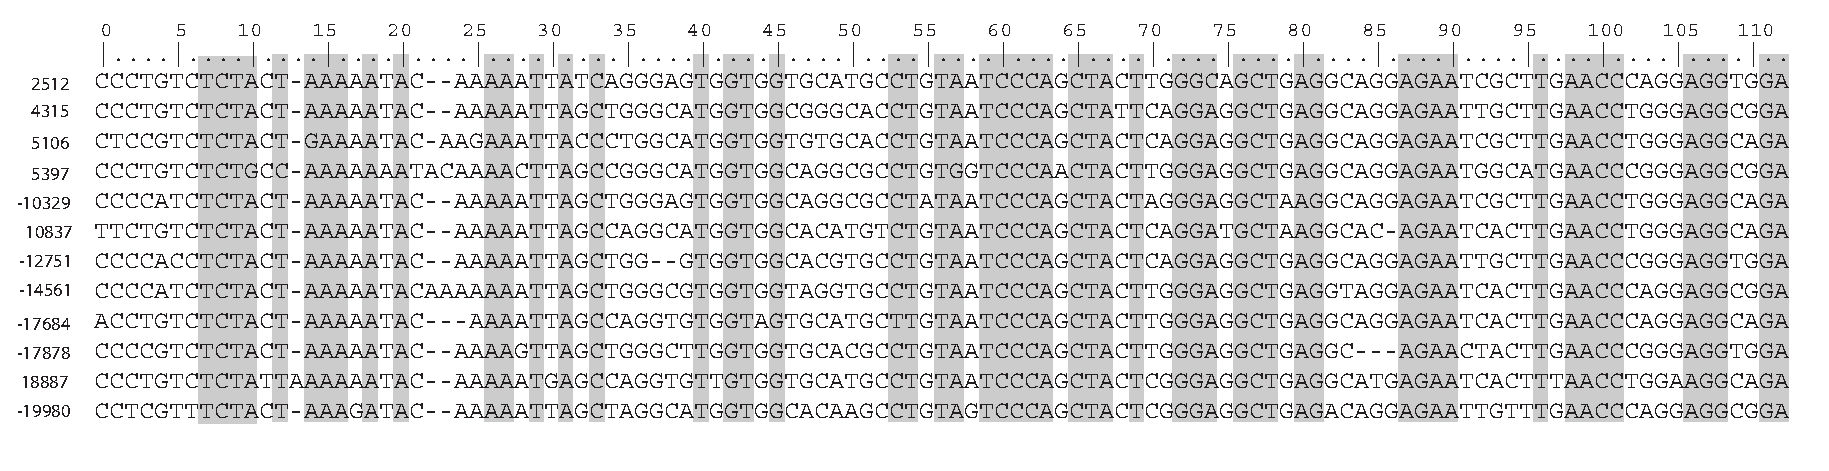
\epsfig{file=./figures/alu_align.eps,width=5.0in}
\caption{Partial alignment of Alu repeat found in the \emph{H. sapiens} BAC clone RP11-355H10 (Accession AC010145.10). Each row represents an aligned ALU. Highlighted columns indicate conserved sequence among all all 12 sequences. Start positions are shown to the left, negative values indicate complement strand.  Local multiple alignment was generated with \texttt{procrastAlign} with parameters: \texttt{--z=9 --w=50}.  }
\label{fig-align}
\end{figure}

\section{Discussion}
We have presented a sensitive and efficient heuristic for local multiple alignment. We have extended our previous results by converting chains of ungapped multi-matches into gapped local multiple alignments. Our method is based around an efficient heuristic for local multiple alignment, featuring a novel method for gapped extensions joining global multiple alignment with a hidden Markov model based homology test.  Experimental results demonstrate that the described method offers a level of alignment accuracy far exceeding that of previous methods.

Further improvement of the alignment methodology will likely require increasingly sensitive methods for seed matching in conjunction with a statistical methodology to assign significance to local multiple alignments.  One possible avenue to increase seed matching sensitivity would be merging overlapping seed matches into a shorter, higher multiplicity match.  A second avenue would be use of palindromic seed families instead of using individual seed patterns. With increased seed matching sensitivity comes additional false positive seed hits, so a statistical test for rejecting insignificant local alignments will likely be required.  Exact computation of $p$-values for local multiple alignments remains a daunting challenge, although fast approximation methods for pairwise alignments have shown promise\cite{repseek} and potentially can be extended to multiple alignments\cite{ref-related1}.

\subsection{Implementation}
We have implemented our method in a program, \texttt{procrastAligner}, available for Linux, Windows, and Mac OS X. Our open-source implementation is available as C++ source code licensed under the GPL.

\section{ Acknowledgments }
The authors would like to thank Yu Zhang for providing the \texttt{eulerAlign} program. We are grateful to Guillaume Achaz for helpful discussions on the gapped extension algorithm. Accuracy evaluations utilized a compute resource grant from the Australian Partnership for Advanced Computing.  AED was supported by NSF grant DBI-0630765. TJT was
supported by Spanish Ministry MECD Grant TIN2004-03382 and AGAUR
Training Grant FI-IQUC-2005.


\bibliographystyle{ws-procs9x6}
\bibliography{procrastination}

\end{document}
